\documentclass{article}
\usepackage{subfigure,graphicx}

\title{Clustering of Time Series using Wavelet Transformations as a Feature Extraction Mechanism}
\author{\textsf{Kathy Norman, Ssurey Moon, Felix Huang, Josu\'e Kuri}\\UCSC Extension. 30164:(003) Machine Learning and Data Mining}

\begin{document}
\maketitle

\section{Introduction}
A time series is a sequence of data points indexed by time at regular intervals. This model is used to represent a wide range of metrics such as the daily closing price of stocks, temperature, precipitation, population, etc. In the context of machine learning and data mining, clustering of a large set of time series is an exploratory technique aimed at identifying and understanding underlying patterns.

Considering every point of a time series as a dimension results in a high dimensional space which clustering algorithms cannot handle easily. These algorithms depend on a distance measure as a basis to maximize cohesion and separation. In a high dimensional space, the contrast between the nearest and the farthest neighbor becomes smaller making it difficult for clustering algorithms to find meaninful groups \cite{BGRS99}.

Data dimensionality reduction is an approach to map a high dimensional space into a lower dimensional space such that the main characteristics of the data points in the original space are preserved and clustering on the lower dimensionality space results in meaningful groups. The two types of dimensionality reduction are feature selection and feature extraction. The former consists in selecting a subset of features from the original features. Feature extraction, on the other hand, generates a new set of features through a mapping function.

Feature extraction techniques commonly used include Singular Value Decomposition (SVD), Discrete Fourier Transform (DFT) and Discrete Wavelet Transform (DWT). Of these techniques, SDV is the most effective at reconstructing time series with minimal error. However, its time complexity $O(mn^2)$, where $m$ is the number of time series and $n$ is the lenght of each time series, makes this a computally-intensive approach \cite{ZHZL06}. A Fast Fourier Transform (FFT) algorithm can compute DFT coefficients in $O(mn \log n)$ and DWT, using a spacial type of wavelet called {\em Haar wavelet} can achieve $O(mn)$ \cite{ZHZL06}.

In this project we use a feature extraction approach based on DWT using the Haar wavelet as the basis for the transformation. We create a generic framework for clustering of time series using this approach and apply the framework to three types of time series: daily closing stock prices, daily values of exchange rates, and earthquake activity over time for various geographic regions. We use a silhouette coefficient as the criterion to evaluate the quality of the clusterings generated by the framework.


\section{Wavelet transformation}

Wavelet transformation is a time-frequency domain transformation technique for hierarchical decomposition of signals \cite{C92,D92}. The decomposition creates an approximation of the original signal that preseves the trend of the signal, as well as additional data sets that provide increasing levels of detail to reconstruct the original signal. This original signal can be reconstructed without loss of information by applying an inverse wavelet transform to the combination of the approximation signal and all the detail data sets.

Early work on wavelets originated with Morlet in the 1980s as a new tool for seismic signal analysis \cite{MAFG82}. Further work by Morlet, Grossman, Meyer, Mallat and Daubechies \cite{CGT89,D88} broght the concept to the mainstream mathematics community with applications in signal processing, statistics and other areas. There is at present a vast body of literature about the foundations and applications of wavelets. The interested reader is referred to \cite{BGG98} and similar works for a comprehensive presentation of the field.


\section{Wavelet-based feature extraction}

Lorem ipsum dolor sit amet, consectetur adipiscing elit, sed do eiusmod tempor incididunt ut labore et dolore magna aliqua. Ut enim ad minim veniam, quis nostrud exercitation ullamco laboris nisi ut aliquip ex ea commodo consequat. Duis aute irure dolor in reprehenderit in voluptate velit esse cillum dolore eu fugiat nulla pariatur. Excepteur sint occaecat cupidatat non proident, sunt in culpa qui officia deserunt mollit anim id est laborum.


\section{Experimental evaluation}

Lorem ipsum dolor sit amet, consectetur adipiscing elit, sed do eiusmod tempor incididunt ut labore et dolore magna aliqua. Ut enim ad minim veniam, quis nostrud exercitation ullamco laboris nisi ut aliquip ex ea commodo consequat. Duis aute irure dolor in reprehenderit in voluptate velit esse cillum dolore eu fugiat nulla pariatur. Excepteur sint occaecat cupidatat non proident, sunt in culpa qui officia deserunt mollit anim id est laborum.

\subsection{Evaluation criteria}

\subsection{Data description}

\subsubsection{Stock closing prices}
\subsubsection{Historic exchange rates}
\subsubsection{Historic earthquake data}


\subsection{Performance evaluation}

\begin{figure}
\begin{center}
\subfigure[Level 2]{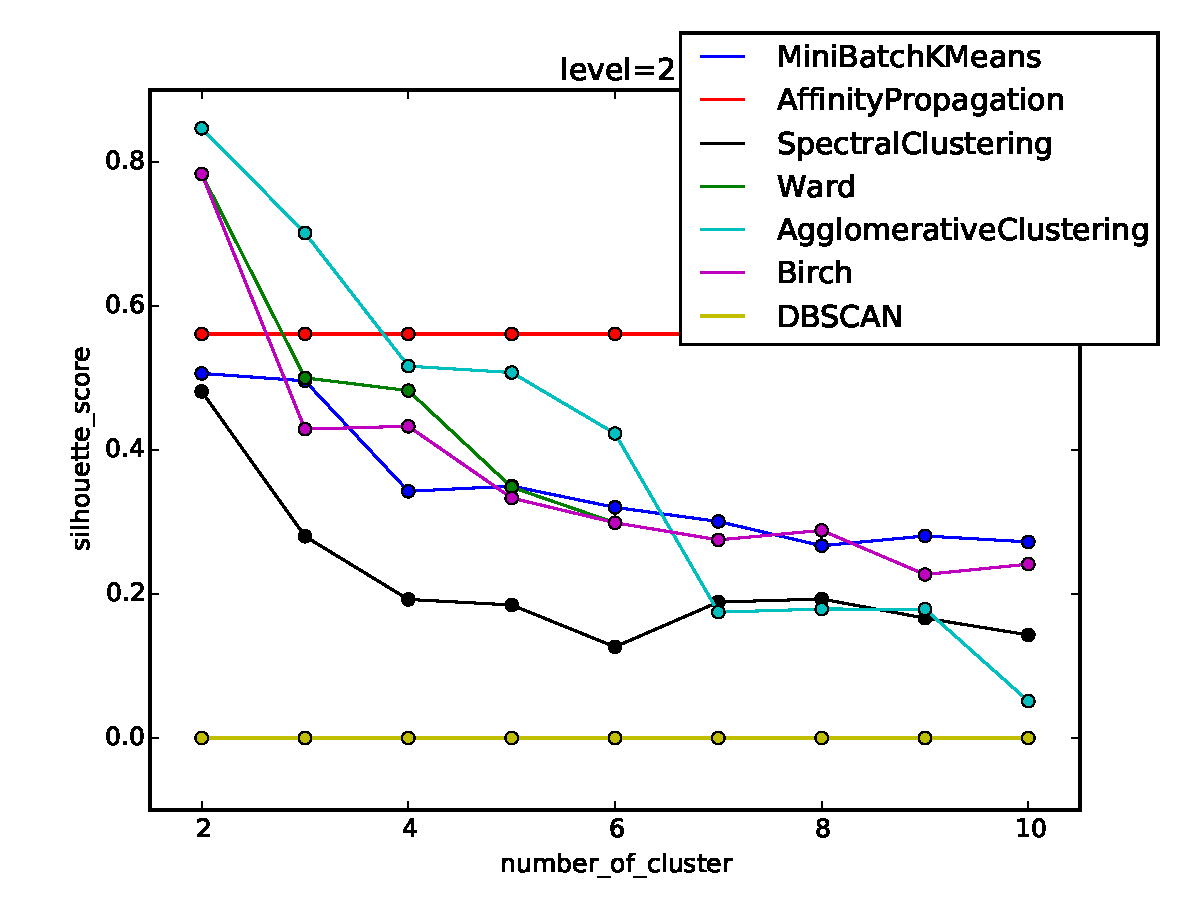
\includegraphics[width=0.49\textwidth]{../task4/silhouette_score_plot_per_number_of_cluster(level=2).pdf}}
\subfigure[Level 4]{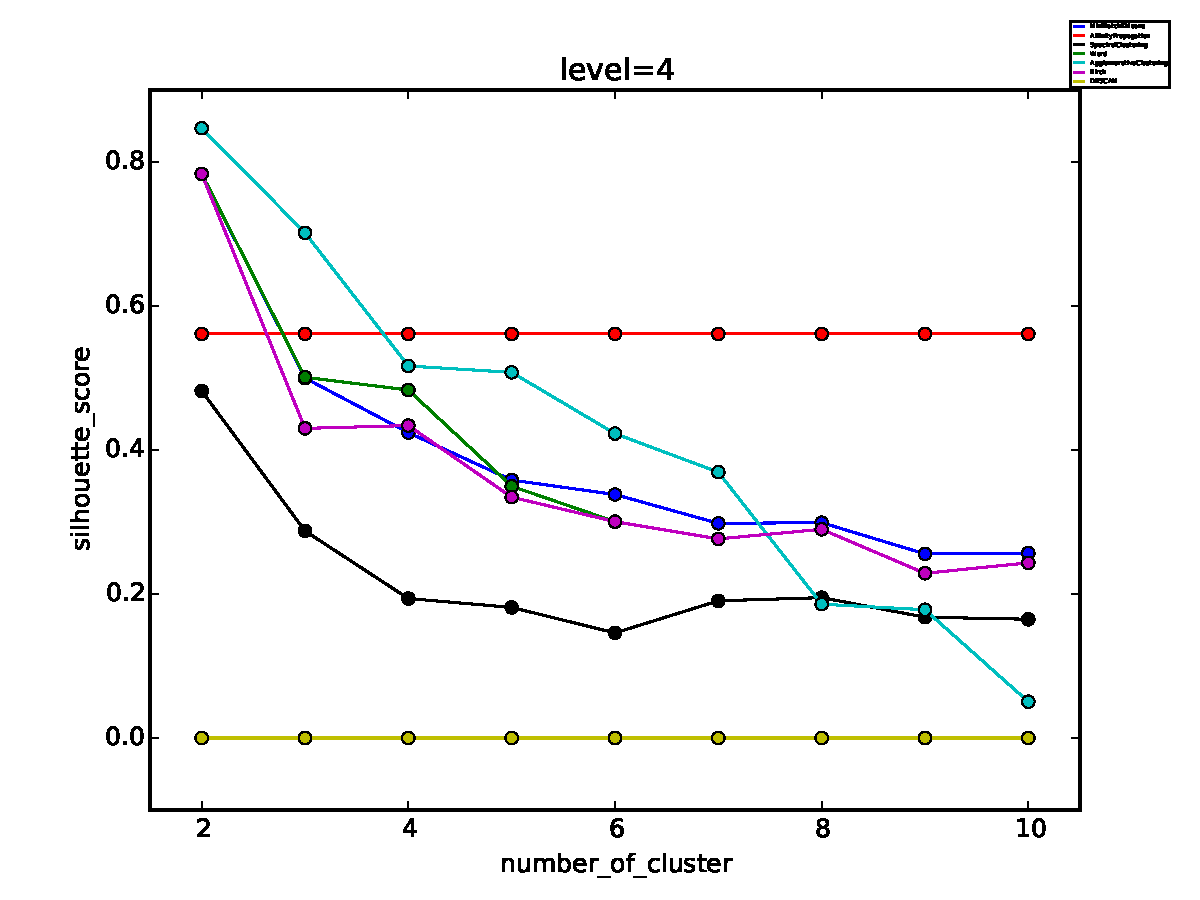
\includegraphics[width=0.49\textwidth]{../task4/silhouette_score_plot_per_number_of_cluster(level=4).pdf}}
\subfigure[Level 6]{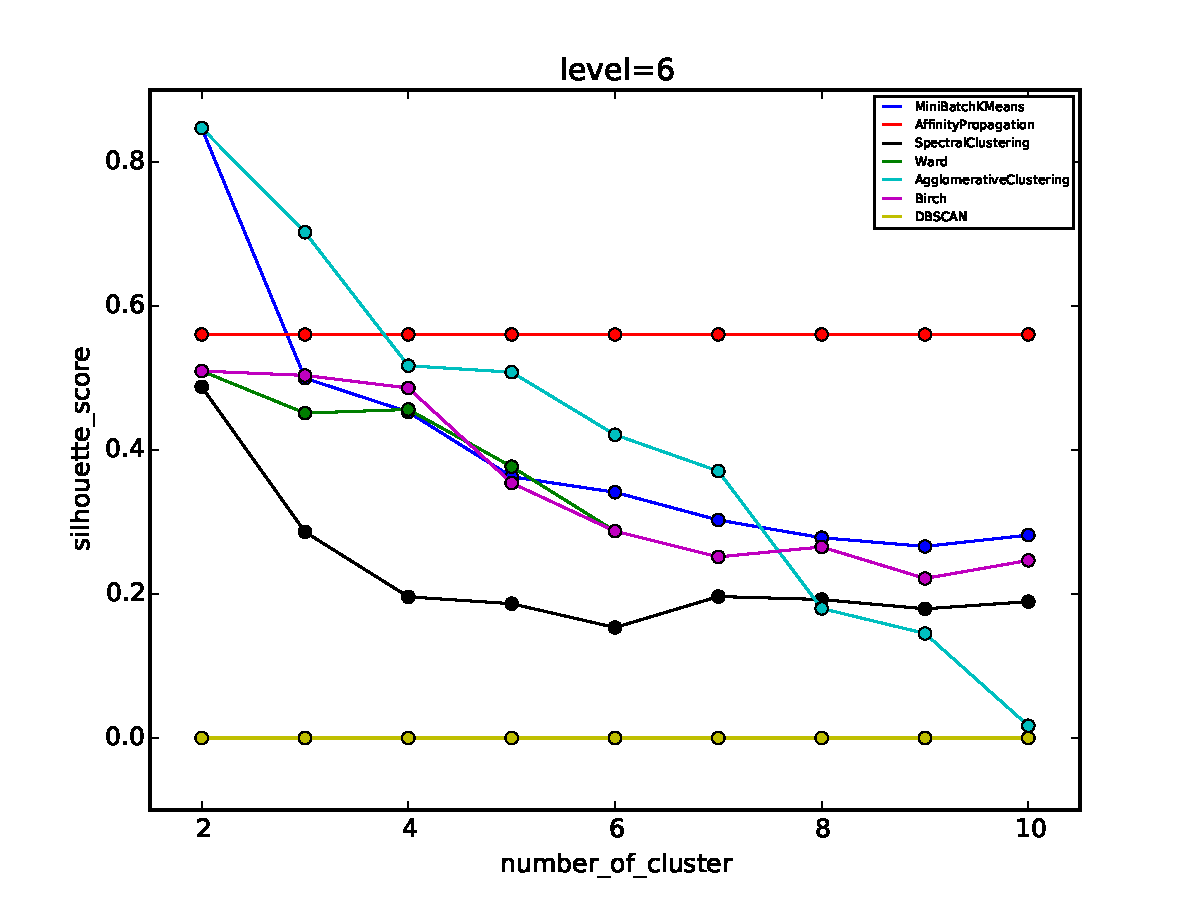
\includegraphics[width=0.49\textwidth]{../task4/silhouette_score_plot_per_number_of_cluster(level=6).pdf}}
\subfigure[Level 8]{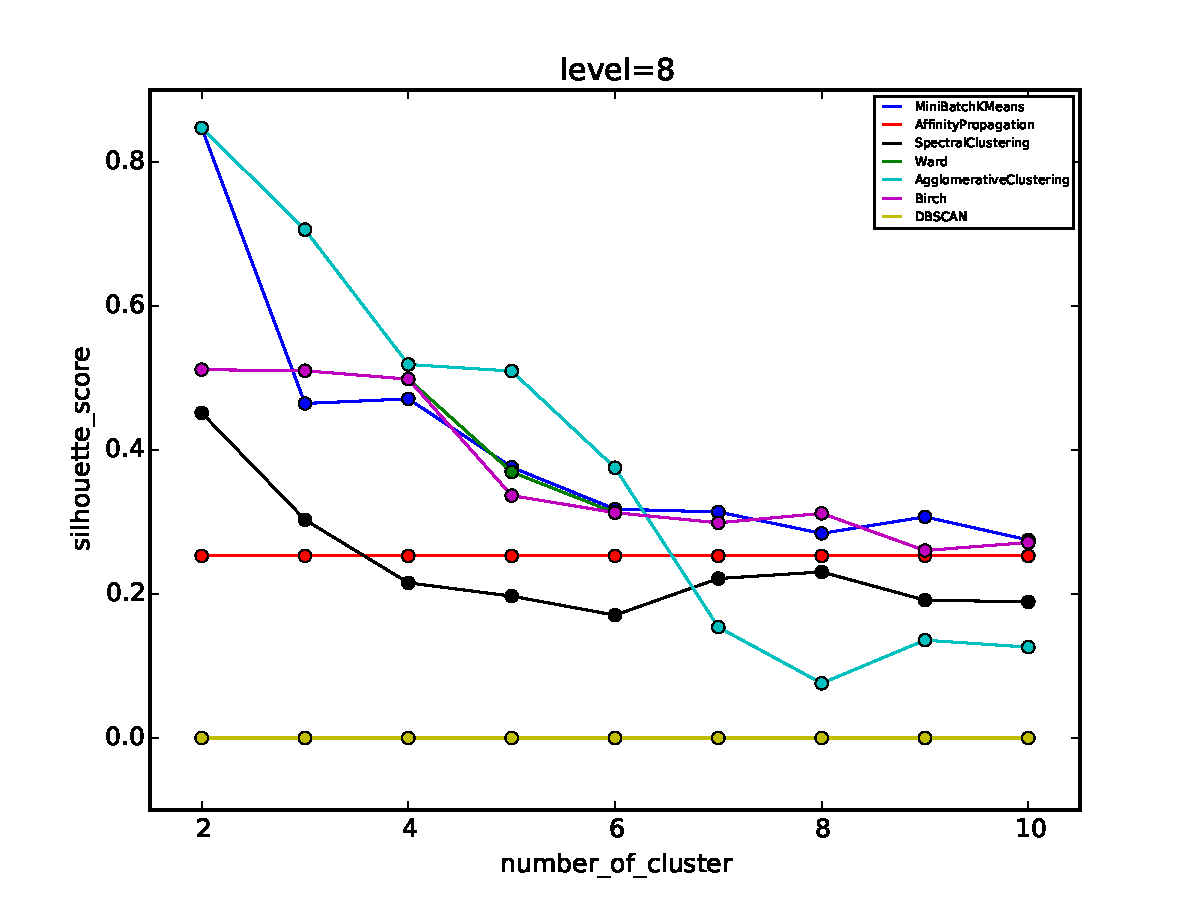
\includegraphics[width=0.49\textwidth]{../task4/silhouette_score_plot_per_number_of_cluster(level=8).pdf}}
\caption{Silhouette score for various clustering levels.} \label{silhouette_levels}
\end{center}
\end{figure}


\begin{figure}
\begin{center}
\subfigure[Two clusters]{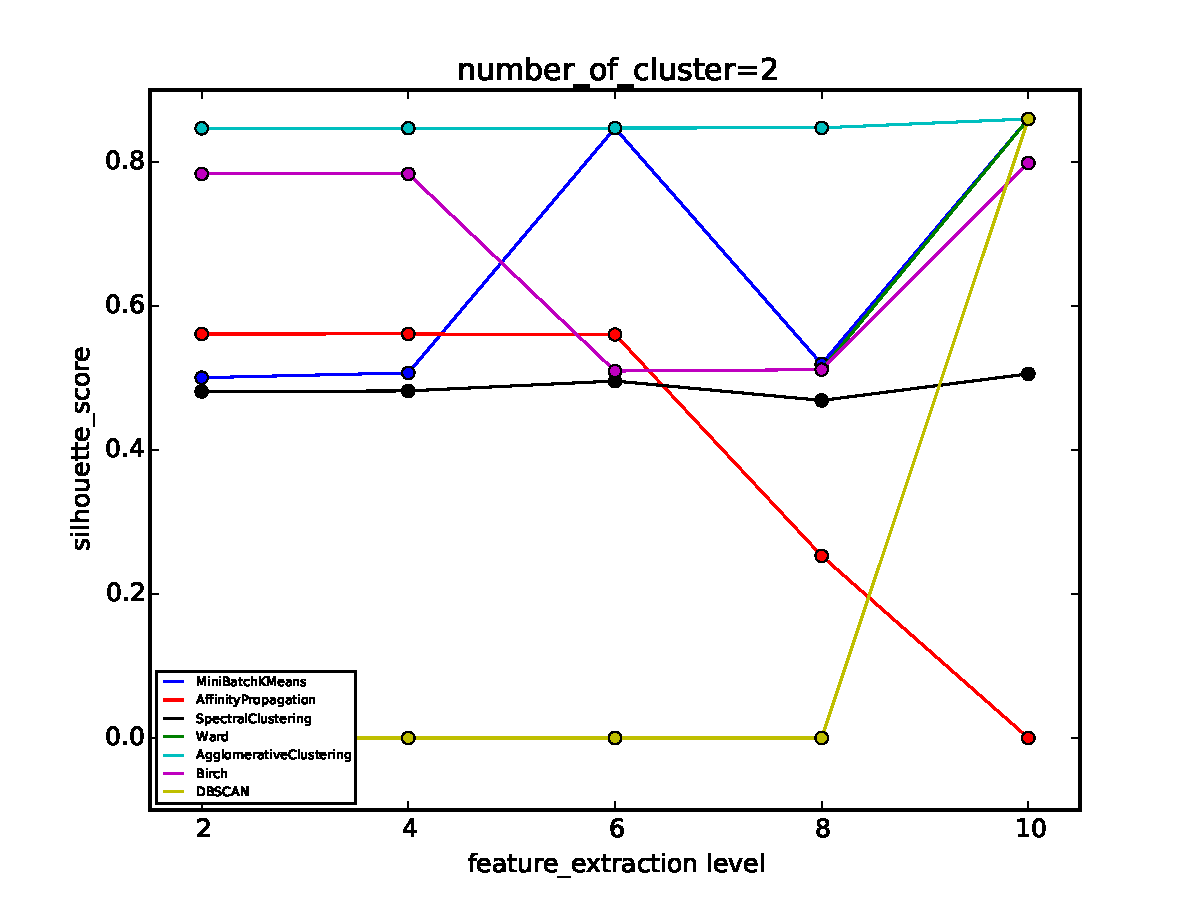
\includegraphics[width=0.49\textwidth]{../task4/silhouette_score_plot_per_level_(clusters=2).pdf}}
\subfigure[Three clusters]{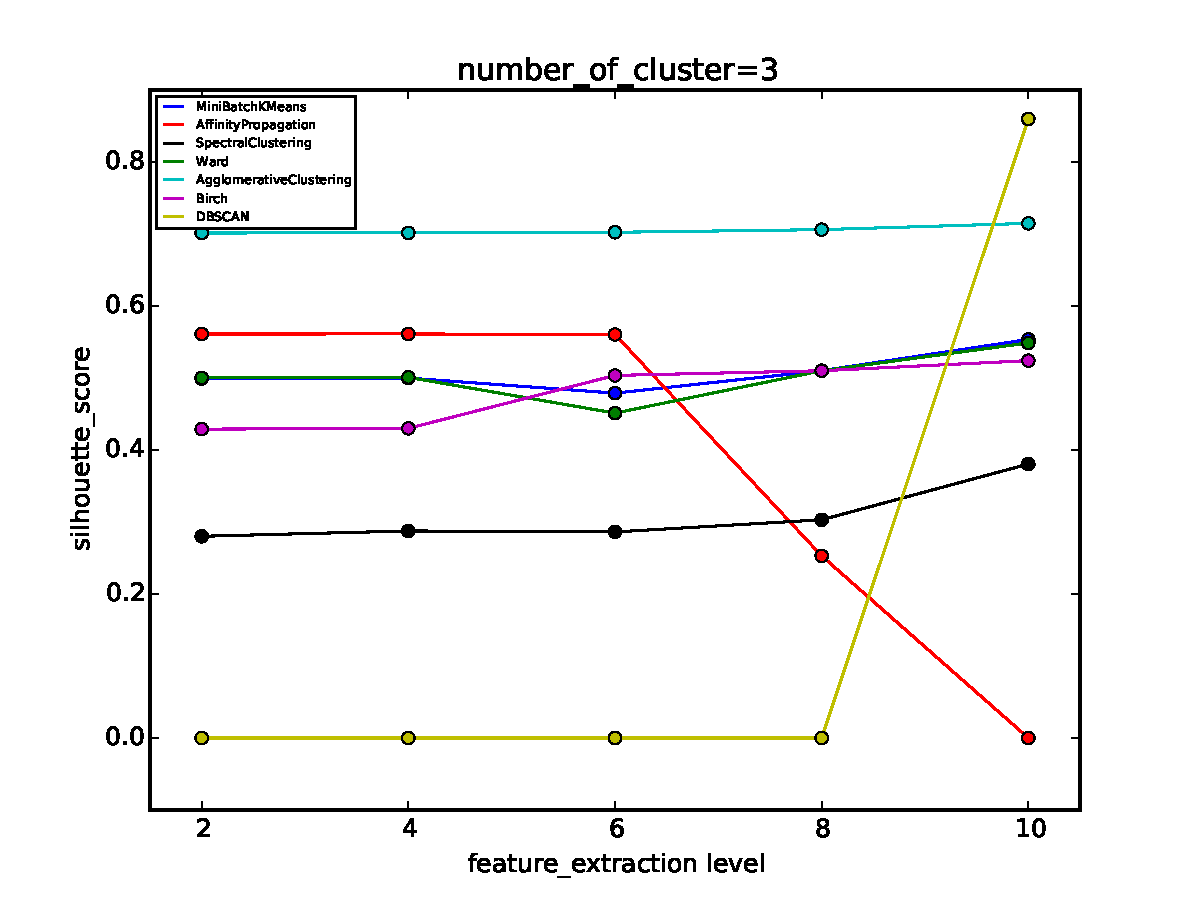
\includegraphics[width=0.49\textwidth]{../task4/silhouette_score_plot_per_level_(clusters=3).pdf}}
\subfigure[Four clusters]{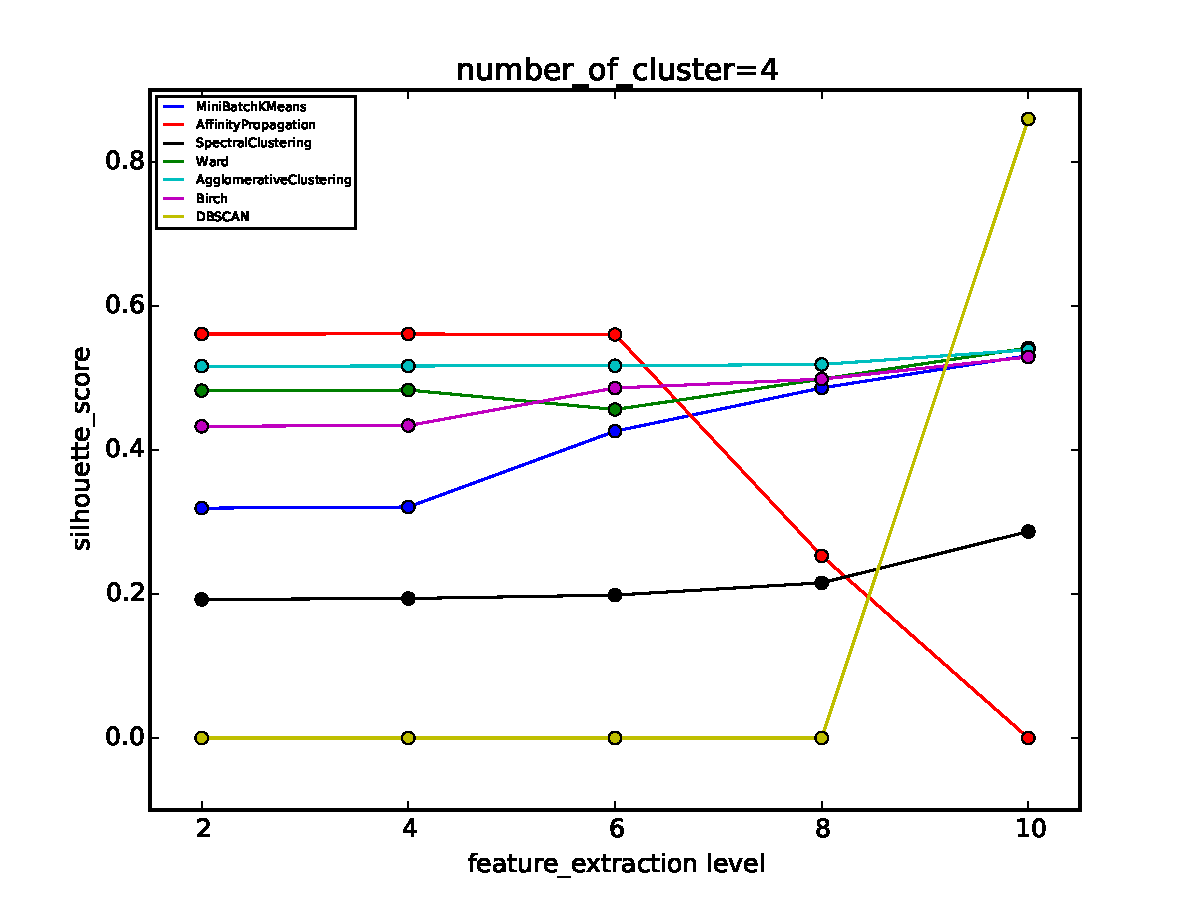
\includegraphics[width=0.49\textwidth]{../task4/silhouette_score_plot_per_level_(clusters=4).pdf}}
\subfigure[Five clusters]{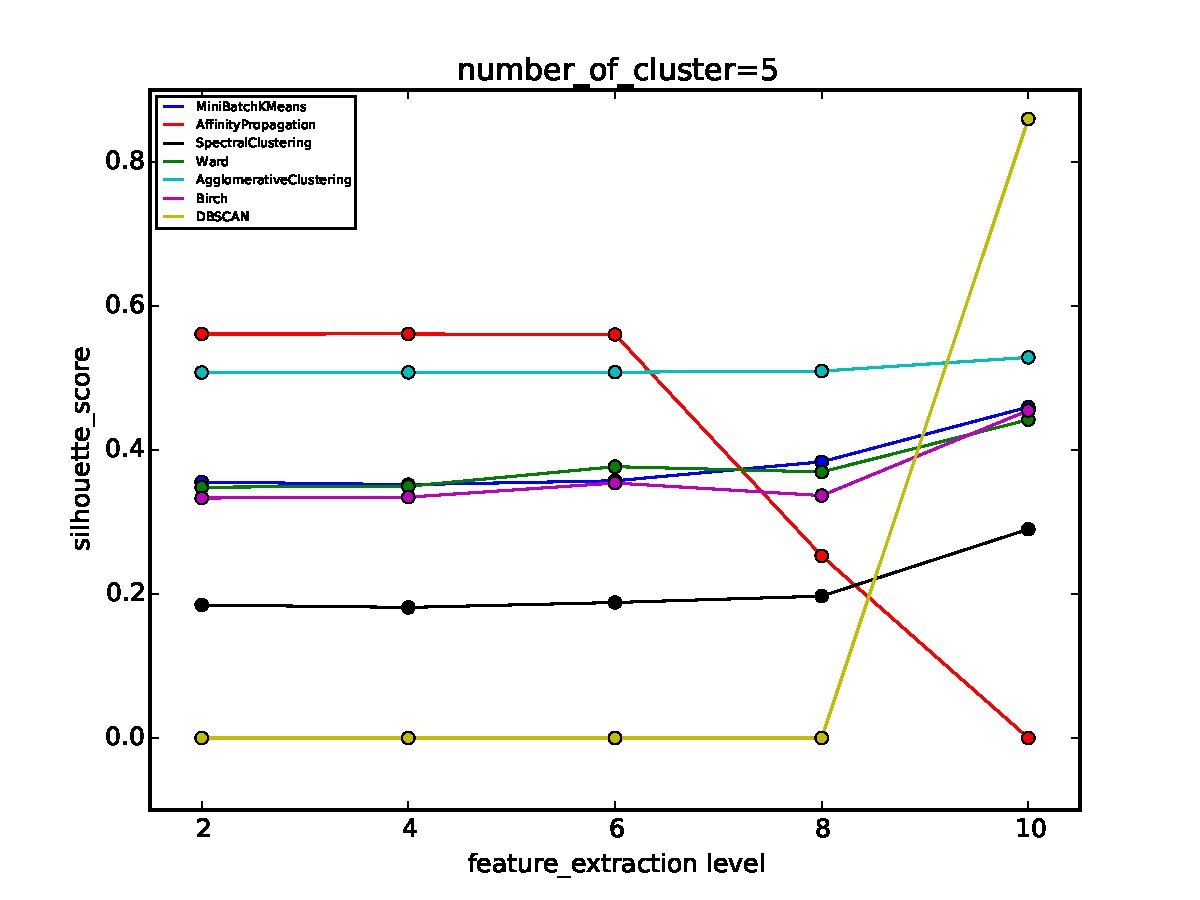
\includegraphics[width=0.49\textwidth]{../task4/silhouette_score_plot_per_level_(clusters=5).pdf}}
\subfigure[Six clusters]{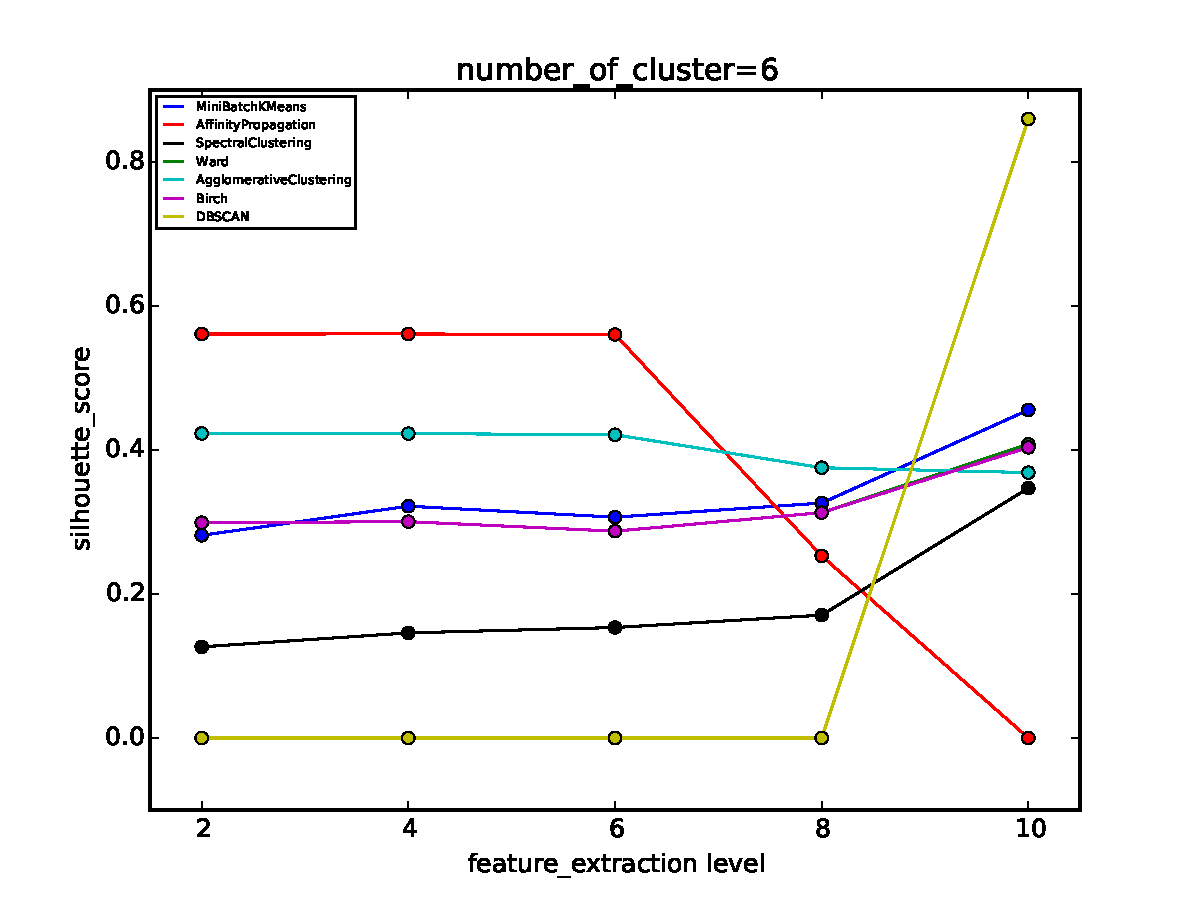
\includegraphics[width=0.49\textwidth]{../task4/silhouette_score_plot_per_level_(clusters=6).pdf}}
\subfigure[Seven clusters]{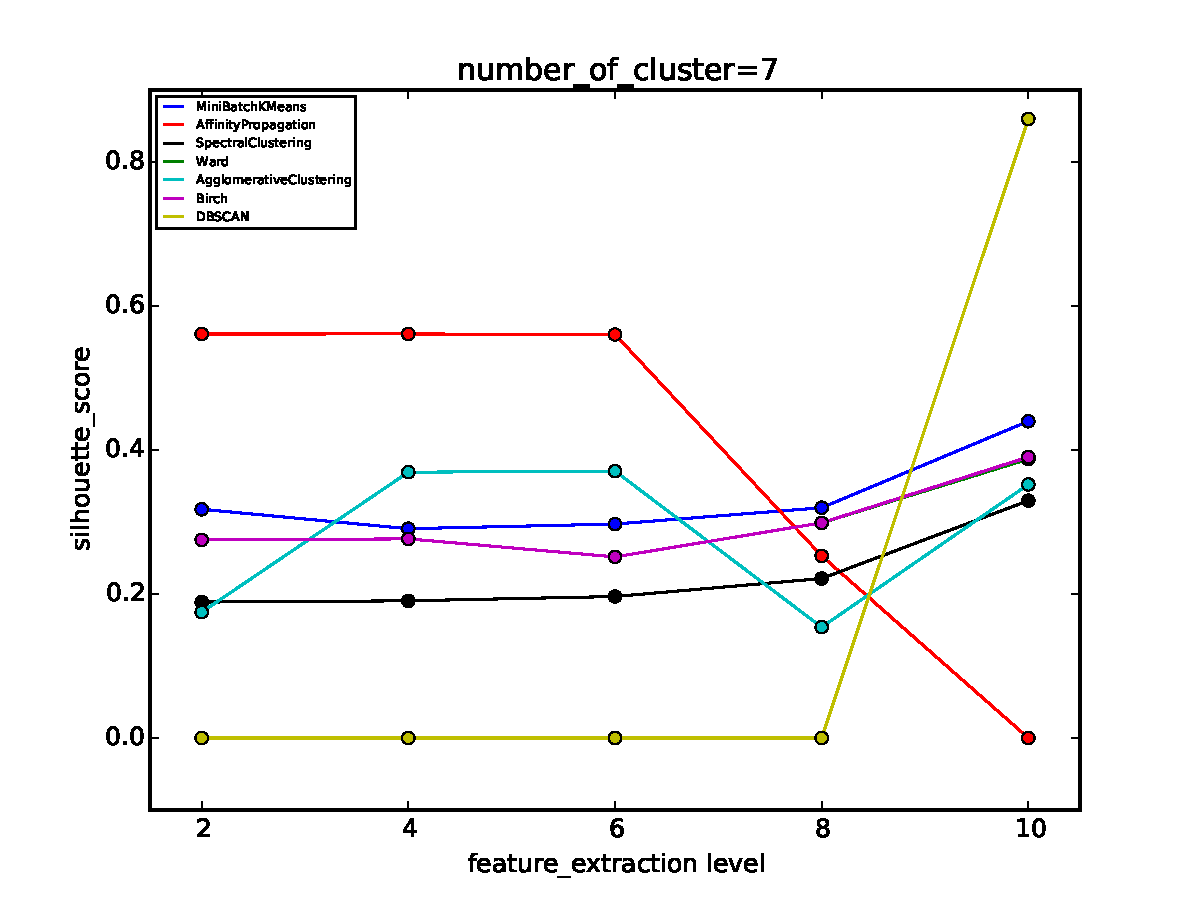
\includegraphics[width=0.49\textwidth]{../task4/silhouette_score_plot_per_level_(clusters=7).pdf}}
\subfigure[Eight clusters]{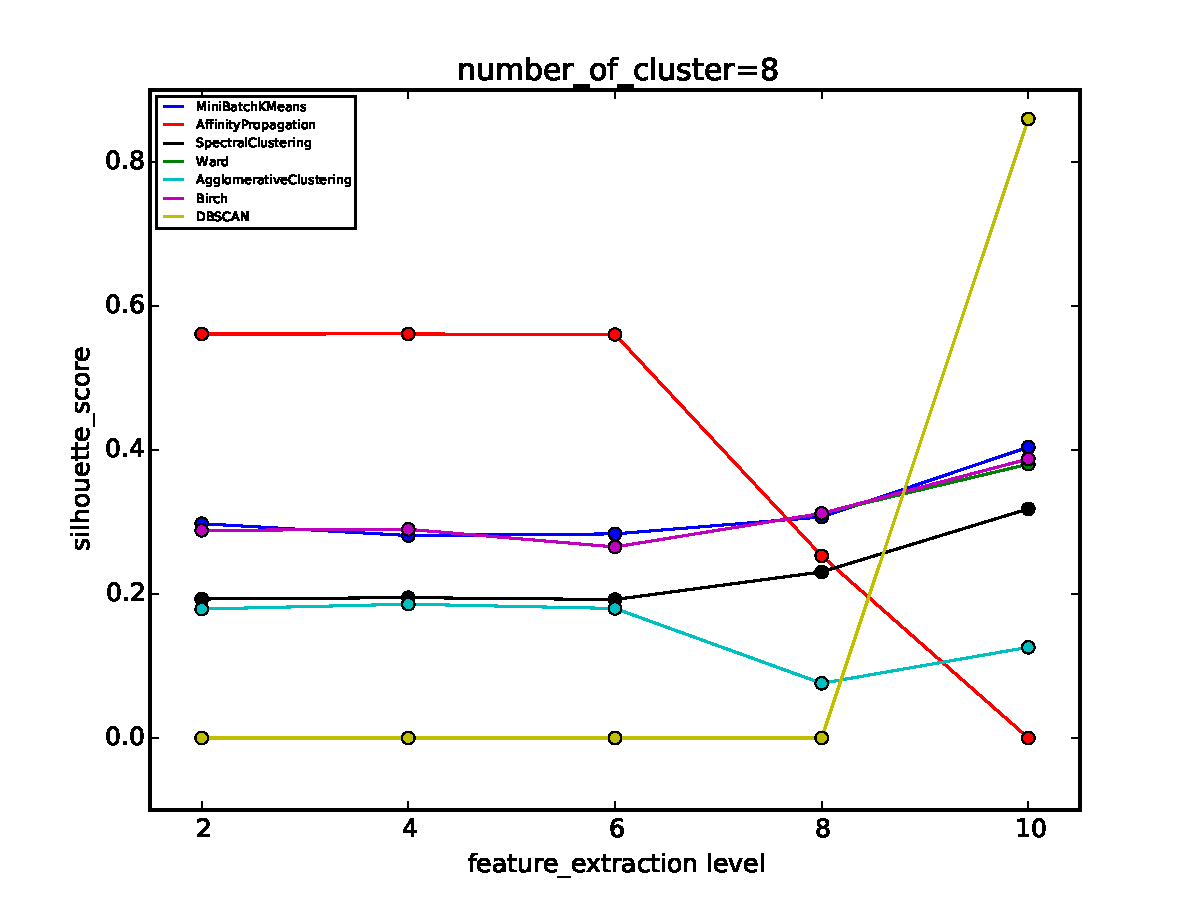
\includegraphics[width=0.49\textwidth]{../task4/silhouette_score_plot_per_level_(clusters=8).pdf}}
\subfigure[Nine clusters]{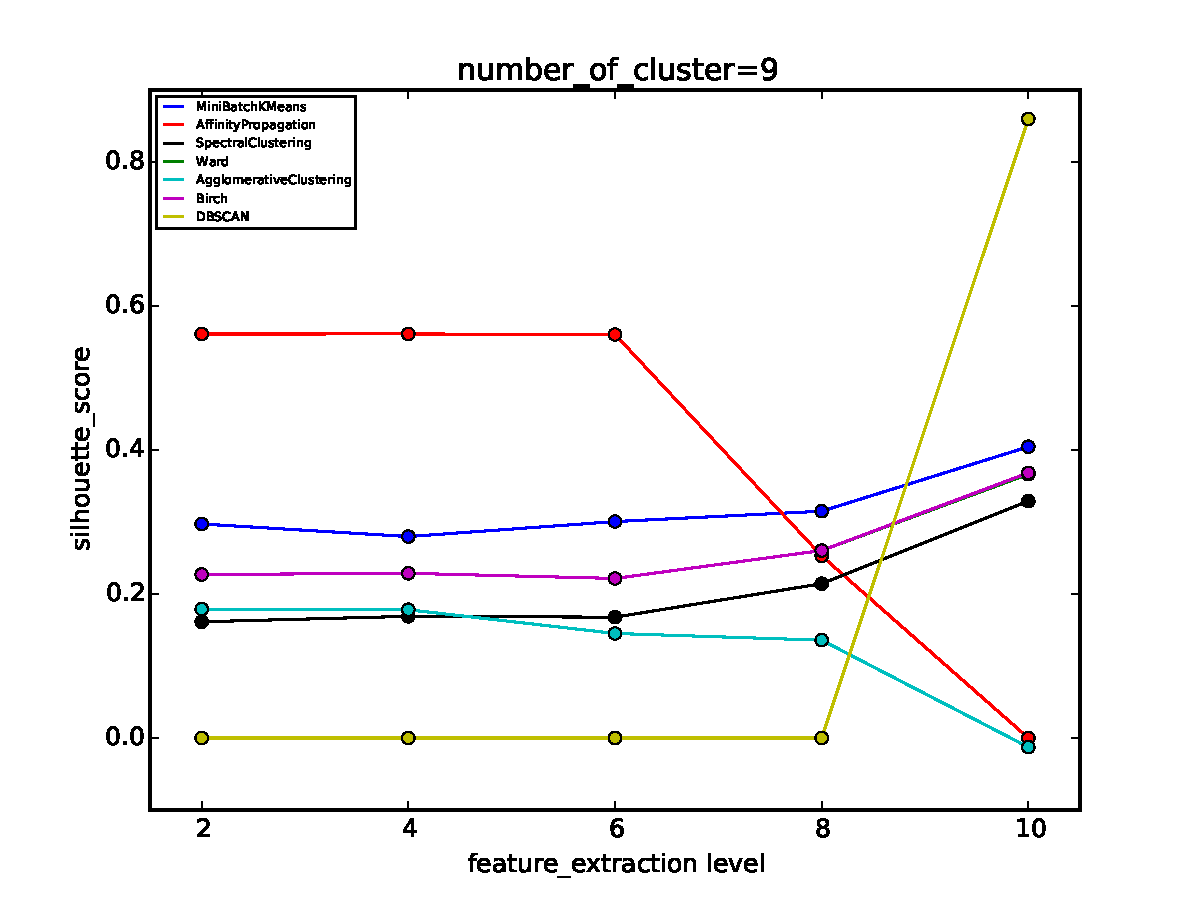
\includegraphics[width=0.49\textwidth]{../task4/silhouette_score_plot_per_level_(clusters=9).pdf}}
\caption{Silhouette score for various clustering levels.} \label{silhouette_levels}
\end{center}
\end{figure}


\section{Conclusions}
Lorem ipsum dolor sit amet, consectetur adipiscing elit, sed do eiusmod tempor incididunt ut labore et dolore magna aliqua. Ut enim ad minim veniam, quis nostrud exercitation ullamco laboris nisi ut aliquip ex ea commodo consequat. Duis aute irure dolor in reprehenderit in voluptate velit esse cillum dolore eu fugiat nulla pariatur. Excepteur sint occaecat cupidatat non proident, sunt in culpa qui officia deserunt mollit anim id est laborum.


  \begin{thebibliography}{1}

\bibitem{BGRS99} K. Beyen, J. Goldstein, R. Ramakrishnan, and U. Shaft. When is nearest neighbor meaningful? In {\em Proceedings of the 7th International Conference on Database Theory}, pp. 217-235, 1999.

\bibitem{ZHZL06} H. Zhang, T. B. Ho, Y. Zhang, M.-S. Lin. Unsupervised Feature Extraction for Time Series Clustering Using Orthogonal Wavelet Transform In {\em Informatica}, Volume 30, pp. 305-319, 2006.

\bibitem{C92} C. K. Chui. {\em An Introduction to Wavelets.} Academic Press, San Diego, 1992.

\bibitem{D92} I. Daubechies. Ten Lectures on Wavelets. {\em SIAM}, Philadelphia, PA, 1992.

\bibitem{MAFG82} J. Morlet, G. Arens, E. Fourgeau and D. Giard. Wave propagation and sampling theory, Part 1: Complex  signal land scattering in multilayer media. {\em Journal of Geophysics,} 47:203-221, 1982.

\bibitem{CGT89} J. M. Combes, A. Grossman and P. Tchamitchian, editors. {\em Wavelets, Time-Frequency Methods and Phase Space.} Springer-Verlag, Berlin 1989.

\bibitem{D88} I. Daubechies. Orthonormal bases of compactly supported wavelets. {\em Communications on Pure and Applied Mathematics,} 41:909-996, 1988.

\bibitem{BGG98} C. Sidney Burrus, R. A. Gopinath, and H. Guo, {\em Introduction to Wavelets and Wavelet Transforms: A Primer,} Prentice Hall, NJ 1998.


\end{thebibliography}

\end{document}